\documentclass[11pt,a4paper, 
swedish,english %% Make sure to put the main language last!
]{article}
\pdfoutput=1

%% Andréas's custom package 
%% (Will work for most purposes, but is mainly focused on physics.)
\usepackage{../custom_as}

%% Figures can now be put in a folder: 
\graphicspath{ {figures/} %{some_folder_name/}
}

%% If you want to change the margins for just the captions
\usepackage[margin=10 pt]{caption}

%% To add todo-notes in the pdf
\usepackage[%disable  %%this will hide all notes
]{todonotes} 

%% Change the margin in the documents
\usepackage[
%            top    = 3cm,              %% top margin
%            bottom = 3cm,              %% bottom margin
%            left   = 3cm, right  = 3cm %% left and right margins
]{geometry}


%% If you want to chage the formating of the section headers
%\renewcommand{\thesection}{...}
\swapcommands{\Lambda}{\varLambda}
\swapcommands{\Omega}{\varOmega}
\swapcommands{\Gamma}{\varGamma}
\newcommand{\Lsq}[1]{\ensuremath{\mathcal{L}^2_{#1}}}
\newcommand{\RT}{\ensuremath{R_{\text{T}}}}
\newcommand{\RH}{\ensuremath{R_{\text{H}}}}

%%%%%%%%%%%%%%%%%%%%%%%%%%%%%%%%%%%%%%%%%%%%%%%%%%%%%%%%%%%%%%%%%%%%%%
\begin{document}%% v v v v v v v v v v v v v v v v v v v v v v v v v v
%%%%%%%%%%%%%%%%%%%%%%%%%%%%%%%%%%%%%%%%%%%%%%%%%%%%%%%%%%%%%%%%%%%%%%


%% If you want to use an external file for the title page
%\input{titlepages.tex}


%%%%%%%%%%%%%%%%%%%% vvv Internal title page vvv %%%%%%%%%%%%%%%%%%%%%
\begin{titlepage}
\title{\tt Project lambda}
\author{Niklas Renström \and Andréas Sundström}
\date{\today}

\maketitle

%% Page numbering:
%\pagenumbering{roman} %% roman pagenumbering
\thispagestyle{empty} \pagestyle{empty} %% no page numbers 

%% The abstract of the document
\begin{abstract} 


\end{abstract}
\newpage
\tableofcontents
\end{titlepage}

\pagenumbering{arabic}
\setcounter{page}{1}
%%%%%%%%%%%%%%%%%%%% ^^^ Internal title page ^^^ %%%%%%%%%%%%%%%%%%%%%
%% If you want a list of all todos
%\todolist


\section{Introduction}
%\todo[inline]{General intro to hyopthermia and freq dep.}

The current hyperthermia treatments mainly utilizes signals consisting of single or a narrow band (NB) of frequencies since simulations and numerical studies have not shown an increase of efficacy by using a wide band (WB). 
However, in mathematical theory there exists a number of uncertainty  principals stating that a function cannot be highly localized in the space and frequency domains at the same time which would encourage the use of a wide band of frequencies, in contrast to prior studies.

This project aims to shed some light to this apparent inconsistency by taking a closer look at relevant uncertainty principles and applying them to a simplified case of scalar fields satisfying the wave equation in two dimensions.
First the Heisenberg inequality, a lower limit of the product of the field's variance in the two domains in  will be applied.
Next, to get something more applicable to hyperthermia an uncertainty principle originally developed by D. Slepian, H.J. Landau and H.O. Pollak, which speaks of how well a function limited in frequency can be localized in a bounded region of space. At this point we will also introduce a polar wave decomposition to yield a more straight forward application of the theory than the normal plane wave decomposition.

Finally the results will be discussed from a hyperthermia treatment point of view and we will discuss some of the limitations as well as possible extensions of the theory.


\subsection{Limitations}
The human body contains many different materials and therefore a real hyperthermia treatment planning will often involve numerically solving Maxwell's equations to simulate how the EM-field will look like in the specific case.

Since this project aims to extract what limitations the wave \emph{nature} sets we are not concerned with the actual wave propagation -- instead we ask the question, given a perfect way to create or propogate the EM-field what limits does a narrow band of frequencies and the wave equation set on the optimal distribution in a bounded region?

With this in mind the study is limited to a homogeneous material stretching through all space. The material is assumed lossfree although the case of lossy materials and dampened EM-field's will be discussed briefly in chapter \ref{ch:discussion}.

Further we limit ourselves to 2 dimensions since this suffices to capture the essential wave nature (a circular ring of wavenumbers as opposed to a point in 1 dimension) whilst not overly complicating the mathematics. 
In this space we try to focus the distribution to a simple body, a disk since we believe that most more complicated bodies would yield approximately the same results.

We will also limit our attention to scalar fields, real EM-fields are in fact vectors with certain limitations to its directions which would produce slightly tighter bounds then what we achieved but this was unfortunately beyond the scope of this project.

Finally, for a real hyperthermia treatment it is not the intensity of the EM-field that is of concern but rather its mean-value in time that is of interest. This has major implications for the frequency dependence of the efficacy and will be discussed to some length in chapter \ref{ch:discussion}. However, the main part of this work is concerned with the EM-field itself and not its time mean.


\subsection{Theory}
For each frequency $\omega$ the electric field will have a harmonic timedependence,and can be represented by phasor notation,
\begin{equation}
  \label{eq:phasor}
\vb*E(\vb*x,t)=\Re\qty[\vb*E(\vb*x)\ee^{-\ii\omega t}]%\cos(\omega t).
\end{equation}
%which allows the use of phasors,
%\begin{equation}
%\vb*E(\vb*x,t)=\Re\qty[\vb*E(\vb*x)\ee^{-\ii\omega t}].
%\end{equation}
In a loss-less and source-less homogeneous media the Maxwell equations reduce to
\begin{equation}
\begin{cases}
\laplacian  \vb*E + k^2\vb*E=0,\\
\div\vb*E = 0,
\end{cases}
\end{equation} 
where $k^2 = \omega^2/v^2$ with $v=\frac{1}{\sqrt{\mu \epsilon}}$ being the speed of propagation. 

To simplify matters however, we will limit the scope of this project to scalar fields satisfying the Helmholtz equation
\begin{equation}
  \label{eq:Helmholtz}
  \qty(\laplacian + k^2)E=0.
\end{equation} 

\subsubsection{Plane wave decomposition}
One solution to the Helmoholtz equation \eqref{eq:Helmholtz} are the plane waves
\begin{equation}\label{eq:plane-wave}
E(\vb*x)=A \ee^{\ii\vb*k \cdot \vb*x},
\end{equation}
were the wavevector $\vb*k$ is any vector such that $\vb*k\vdot\vb*k=k^2$, and $A$ is a constant amplitude. 

The next step is to allow more for more than one frequency. The solution for each frequency will be of the form \eqref{eq:plane-wave}, each with its own amplitude $A(\vb*k)$. These solutions can then be summed up over all frequencies (magnitude as well as directions of $\vb*k$) and the final $E$ field becomes\footnotemark{}
%\begin{equation} \label{eq:gen_sol}
% E(\vb*x)=\int%_{\abs{\vb*k}=\frac{\omega}{v}}
% \vb*A(\vb*k)\ee^{\ii\vb*k\cdot\vb*x}\id^3k,
%\end{equation}
%where the vectoramplitude $\vb*A(\vb*k)$ now represents the amplitude of each wavecomponent $\ee^{\ii\vb*k \cdot \vb*x}$.
%The EM-field can also be expanded by its Fourier Transform
\begin{equation} \label{eq:f_exp}
E(\vb*x)= (2\pi)^{-D} \oldint_{\vb*k} \rd^Dk\,
A(\vb*k) \ee^{\ii\vb*k\cdot\vb*x}.
\end{equation}
\footnotetext{The factor of $(2\pi)^{-D}$ is just for convenience in the comparison with the $D$ dimensional Fourier transform.}

We can now identify \eqref{eq:f_exp} as an inverse Fourier transform of $A(\vb*k)$, and thus $A(\vb*k)$ has to be the Fourier transform of $E(\vb*x)$.
%Comparing the Fourier expansion (\ref{eq:f_exp}), an integral over the whole $\vb*k$-space, with the general solution (\ref{eq:gen_sol}), an integral only over the subspace where $\abs{\vb*k}=\frac{\omega}{v}$ one can identify an expression for the Fourier transform $\widetilde{\vb*E}(\vb*k)$ as
%\begin{equation}
%  \label{eq:f_transf}
%  \widetilde{\vb*E}(\vb*k)=2\pi\vb*A(\vb*k)\delta(\abs{\vb*k}-\frac{\omega}{v})=2\pi\vb*A(\theta,\phi)\delta(\abs{\vb*k}-\frac{\omega}{v}).
%\end{equation}
%Here a $\delta(\abs{\vb*k}-\frac{\omega}{v})$-term has been introduced to display the fact that the Fourier transform $\widetilde{\vb*E}(\vb*k)$ vanishes where $\abs{\vb*k} \neq\frac{\omega}{v}$.
%This is further emphasized in the last step where one sees the amplitude $\vb*A$ not as a function of the wavevector $\vb*k$ but as a function of the angles in the $\vb*k$-space $\theta$ and $\phi$.

%In short, for each frequency $\omega$ the Fourier transform of the EM-field is concentrated to a sphere shell with radius $\abs{\vb*k}=\frac{\omega}{v}$ and vanishes elsewhere.

\subsubsection{Polar wave decomposition in 2 dimensions}
The 2 dimensional Helmholtz equation \eqref{eq:Helmholtz} in polar cooridnats is
\begin{equation}
\label{eq:Helmholtz_polar}
\qty(\pdv[2]{r}+\frac{1}{r}\pdv{r}+\frac{1}{r^2}\pdv[2]{\theta})E+k^2E=0,
\end{equation}
%
%For a separable function $\phi(r,\theta)=R(r)\Theta(\theta)$ the equation separates into
%\begin{align}
%&n^2\Theta+\dv[2]{\Theta}{\theta}=0 \label{eq:angular} \\
%&r^2\dv[2]{R}{r}+r\dv{R}{r}+(k^2r^2-n^2)R=0 \label{eq:radial}.
%\end{align}
%Equation \eqref{eq:angular} has harmonic solutions
%\begin{equation} \label{eq:sol_angular}
%\Theta(\theta)=c_n\ee^{\ii n \theta}.
%\end{equation}
%Since $\Theta$ must be $2\pi$ periodic, $n$ must be an integer. 
%%We notice that these form a base for functions defined on the interval$[0,2\pi)$
%The radial equation \eqref{eq:radial} on the other hand has a solution of Bessel functions
%\begin{equation}
%\label{eq:sol_radial}
%R(r)=a_n J_{n}(kr)+a'_n N_{n}(kr).
%\end{equation}
%We are however only interested in solutions \emph{without} singularities, wherefore only Bessel functions of the first kind are treated. % $a'_n=0$
%%These functions form a base for functions defined on $[0, \infty)$ but the second kind of Bessel function $N_n$  cannot represent any physical function since they have a singularity in 0 and will therefore be disregarded.
%The final solution to \eqref{eq:Helmholtz_polar} can be written as
%\begin{equation*}
%\phi_n(r,\theta)=a_nJ_n(kr)\ee^{\ii n \theta}.
%\end{equation*}
%
%Since the Helmholtz equation is linear, an arbitrary non-singular function satisfying it can be written as a sum 
Which has the standard non-singular solution
\begin{equation}
E(r, \theta)=\sum_{n=-\infty}^{\infty} a_nJ_n(kr)\ee^{\ii n \theta}.
\end{equation}

%The Helmholtz equation \eqref{eq:Helmholtz} is valid for a given frequency $\omega$. To get the EM-field of many different frequency components one has to sum over all of them, or in the continous limit integrate. To integrate over $\omega$ is the same as integrating over $k$ which corresponds to the radius in the Fourier space. To get a direct analog to the circle rings previously discussed we can therefore let $k$ go from $q\Gamma$ to $\Gamma$ and obtain a general EM-field:
Analogously to the plane wave decomposition, we now introduce a spectrum of frequencies, and obtain
\begin{equation}
\label{eq:polar_wave_general}
E(r,\theta)
=\oldint_{k} \rd k \sum_{n=-\infty}^{\infty}\!\!a_n(k) J_n(kr)\ee^{\ii n \theta}
=\sum_{n=-\infty}^{\infty}\!\! \ee^{\ii n \theta} \oldint_{k} \rd{k}\,k\,b_n(k) J_n(kr),
\end{equation}
where in the last step $a_n(k)$ has been replaced with $k\,b_n(k)$ for later convenience.

%\subsubsection{Connection between Fourier and Bessel decomposition}





\section{Focusing meassures}
To start talking about focusing waves, there has to be some meassure
to quantify how well focused a wave is. This report will mainly deal
with the intensity meassure used by Slepian, Landau and Pollack in a
series of papers
\cite{PSWF-I_1961,PSWF-II_1961,PSWF-III_1962,PSWF-IV_1964,PSWF-V_1978}.
However, to address the Heissenberg uncertainty principle, which
concerns a type of variance meassure, an account of both types of
meassures and how they are used will be given in this section. 

%%%%%%%%%%%%%%%%%%%%%%%%%%%%%%%%%%%%%%%%%%%%%%%%%%%%%%%%%%%%%%%%%%%%%%
\begin{comment}
\subsection{Heisenberg's uncertainty principle}
\todo[inline]{REDO!}
The Fourier theory states that any function in space can be divided into a linear combination of plane waves 
\begin{equation*}
 f(\vb*x) = \int_{\vb*k}\id^3k \tilde{f}(\vb*k) \ee^{\ii( \vb*k\vdot\vb*x - \omega t)}
\end{equation*}
with different wave-vectors $\vb*k$. %wavelengths and directions of propagations. 
One can speak of different representations in the space ($\vb*x$) domain and the spacial frequency ($\vb*k$) domain respectively, with the Fourier transform as the link between them.

Heisenberg's uncertainty principle, a famous formula in quantum physics, states that one cannot perfectly determine both the position and momentum of a free particle in space.
This has its root in the fact that the position and momentum of a particle is reltated by a Fourier transform. In a more general sense the Heisenberg uncertainty related the spread in frequency to the spread in time or position.
%This inequality however, is based only on the wave nature of particles and can be seen more as a mathematical inequality on Hilbert spaces than a physical one. As such it also has an equivalent with respect to Fourier transforms which says that the more localized a function is in the space domain the more spread out it must be in the spacial frequency domain.

From Maxwell's equations we know that if an electric field in a lossless media oscillates in time with a certain angular frequency $\omega$ then it  must also oscillate in space with a certain wavevector $k=\sqrt{\mu\epsilon}\omega$. 
%wavelength $\lambda=\sqrt{\epsilon \mu} \omega 2\pi$. Since the wavelength is basically the inverse of the length of the wavvevector $\vb*k$, the Fourier transform would be limited to contain wavevectors with such length. 
An electric field generated by a NB signal will be highly localized in the frequency domain which should lead to a big spread in the spacial domain. Therefore an UWB signal would intuitievely lead to a much more focused field which contradicts previous results [?some~papers?]. We believe that this contradiction is due to a lack of detail in the reasoning and to understand why one must ``put the words into numbers'' and clarify what the uncertainty principle actually says and how it can be applied to the case of hyperthermia.
\end{comment}
%%%%%%%%%%%%%%%%%%%%%%%%%%%%%%%%%%%%%%%%%%%%%%%%%%%%%%%%%%%%%%%%%%%%%%

\subsection{Heisenberg's uncertainty principle}
%\subsubsection{Heisenberg's inequality}
The common quantum mechanical version of Heisenberg's uncertainty
principle used in states that \emph{the product of the variance of
  position and momentum must be greater than some fixed value}. This
is however rooted in the interpretation that position and momentum are
related through fourier transfrom. 

The general mathematical statement of the Heissenberg uncertainty
principle, for a function $f$ and its Fourier transfrom $\tilde{f}$,
is \cite{Folland} 
\todo{Need a value here}
\begin{equation}
\Delta_{\vb*a}f \Delta_{\vb*\alpha} \tilde{f} \geq ?? \quad 
%\forall \vb*a, \vb*\alpha, 
\forall f \in \Lsq{\infty},%[\mathbb{R}^2],
\end{equation}
where $\Delta_{\vb*a}f$ is a variance measure of $f$ is around
\emph{any} reference point $\vb*a$; analogously for
$\Delta_{\vb*\alpha}$ and $\vb*\alpha$.
These variances are defined by
\begin{equation} \label{eq:spread_def}
\Delta_{\vb*a}f=
\frac{\oldint_{\vb*x}\id^3x\abs{\vb*x-\vb*a}^2\abs{f(\vb*x)}^2}
{\oldint_{\vb*x}\id^3x\abs{f(\vb*x)}^2},
\end{equation}
and analogously for the Fourier transfrom.
The minimum is achieved when $\vb*a$ is at the center of mass of $f$.

%For the EM-field this gives an inequality for each component $E_i$\footnotemark{}
%\begin{equation}
%  \label{eq:ineq_final}
%  \Delta_{\vb*a}E_i\geq \frac{9}{4} \frac{1}{\mathrm{Min}_\alpha\Delta_{\vb*\alpha}\tilde{E_i}}, \quad \forall \vb*a.
%\end{equation}
\todo[inline]{Need to rewrite!}
Since the fourier transform of the EM field is concentrated on a sphere we achieve the minimum spread for $\alpha=0$ and using equations \eqref{eq:spread_def} one gets,
$\min_\alpha\Delta_{\vb*\alpha}\tilde{E}=\frac{\omega^2}{v^2}$ and \eqref{eq:ineq_final} becomes
\begin{equation}
 \Delta_{\vb*a}E\geq \frac{9v^2}{4\omega^2}=\frac{9\lambda^2}{16\pi^2}=\frac{9}{16\pi^2\epsilon\mu\nu^2}.
 \end{equation}


If the spacial variation of $f$ is high it implies that it cannot be
highly localized to one single small neighbourhood in space; it does not
however, preclude $f$ from having narrow peaks, there can e.g. exist
several narrow peaks which are spread out from each other and still
have $\Delta{f}$ being large.

For hyperthermia treatment, this means that the variation measure at
best gives a hint on what we want. It is possilbe to achieve a very
strong and narrow radiation peak inside the tumour without violating
the Heissenberg inequality, i.e. using NB signals, as long as a
significant part of the radiation intensity is located outside of the 
head.  
This however is a consequence of the particular focus meassure used in
this uncertainty relation; the mathematical result is still true, but
it might not provide enough insite to be practically applicable in
hyperthermia treatments.



\subsection{The Slepian-Landau-Pollak uncertainty relations}
\todo[inline]{REDO}
In a series of papers from the 60's D. Slepian, H.J. Landau and H.O. Pollak investigated how much energy a frequency-limited function can keep if it is restricted in space. By doing this one can reach an inequality on the form
\begin{equation}
\abs{S}\abs{\Omega} \geq c(\alpha,\beta),
\end{equation}
Where $S$ and $\Omega$ are areas to which a function is restricted to in space respectivley frequency. The constants $\alpha$ and $\beta$ are the fractions of energy that the function contains in these areas. 

In what follows we will show the broad strokes for developing the theory from which the inequality can be extracted. In doing so we will prove the existance of a useful set of functions ${\psi_i}$ who span the room of frequency-limited functions and one of which maximizes the energy retained for a frequency-limited function also limited in the space $S$.

A square-integrable function $f$ of $D$ variables is said to be $\Omega$-limited if it can be represented as a Fourier integral over the bounded region $\Omega$,

\begin{equation}
  f(\vb*x)=\qty(\frac{1}{2\pi})^D\int_\Omega \tilde{f}(\vb*k)\ee^{\ii(\vb*k \cdot \vb*x)} \id^Dk,
\end{equation}
that is, it only contains frequencies in the area $\Omega$.
We define the energy of a function to be
\begin{equation*}
A=\int_{R^D}\abs{f(\vb*x)}^2\id^3x.
\end{equation*}
By Parseval's theorem we get that
\begin{equation*}
A=\int_{R^D}\abs{f(\vb*x)}^2\id^3x=\qty(\frac{1}{2\pi})^D \int_\Omega \abs{\tilde{f}(\vb*k)}^2 \id^Dk.
\end{equation*}
In a bounded region $S$ of the space $R^D$ one gets the total energy
\begin{align*}
  A_S=\int_S\abs{f(\vb*x)}^2\id^Dx&=\int_S\id^Dx \qty(\frac{1}{2\pi})^{2D}\int_\Omega \tilde{f}(\vb*k)\ee^{\ii\vb*k\cdot \vb*x}\id^Dk \int_\Omega \tilde{f}^*(\vb*k')\ee^{-\ii\vb*k'\cdot \vb*x}\id^Dk'\\
 & =\qty (\frac{1}{2\pi})^D \int_\Omega\id^3k\int_\Omega\tilde{f}(\vb*k)\tilde{f}^*(\vb*k')K_s(\vb*k-\vb*k')\id^Dk',
\end{align*}
with the kernel
\begin{equation}
  \label{eq:kernel}
K_s(\vb*k-\vb*k')=\frac{1}{2\pi}^D\int_S\ee^{\ii\vb*x \cdot(\vb*k-\vb*k')}.
\end{equation}
Next if we define an integraloperator $I^{[\Omega S]}$ such that;
\begin{equation}
  \label{eq:int_op}
\qty[I^{[\Omega S]}\phi](\vb*k')=\int_\Omega K_S(\vb*k-\vb*k')\phi(\vb*k)\id^Dk,
\end{equation}
and an inner product on the $\Omega$-space by
\begin{equation}
  \label{eq:in_prod}
   \langle f,g\rangle =\int_\Omega f(\vb*k)g^*(\vb*k)\id^3k,
\end{equation}
the fraction of energy that an $\Omega$-limited function $f$ can have in a region $S$ can be written as
\begin{equation}
  \label{eq:energy_frac_final}
\frac{A_s}{A}=\frac{\int_\Omega\qty[I^{[\Omega S]}\tilde{f}](\vb*k)\tilde{f}^*(\vb*k)\id^Dk}{\int_\Omega \abs{\tilde{f}(\vb*k)}^2 \id^Dk}=\frac{ \langle I\tilde{f}, \tilde{f}\rangle}{\langle \tilde{f}, \tilde{f} \rangle}.
\end{equation}

 In the litterature integral operators of the kind \eqref{eq:int_op} are called Hilbert-Schmidt integral operators if the kernel is square-integrable in $\Omega$, and such an operator is compact. Since the regions $S$ and $\Omega$ are bounded square-integrability holds for the kernel \eqref{eq:kernel} and since it is also complex symmetric with respect to its arguments, $K_s(\vb*k-\vb*k')=K_s^*(\vb*k'-\vb*k)$, the integral operator is self-adjoint with respect to the inner product \eqref{eq:in_prod}. From the Spectral theorem it now follows that the functions fullfilling the eigenvalue equation
\begin{equation}
  \label{eq:eigen}
\qty[I^{[\Omega S]}\psi](\vb*k)=\int_\Omega K_s(\vb*k')\psi(\vb*k') \id^Dk'=\lambda \psi(\vb*k)
\end{equation}
form an orthogonal base for the space $\Omega$ and thus their inverse Fourier transform a base for the space of $\Omega$-limited functions in $R^D$. It also follows that the maximum of equation \eqref{eq:energy_frac_final}, the maximum fraction of energy, equals the largest eigenvalue $\lambda_0$ of equation \eqref{eq:eigen} and the function fulfilling this is the inverse Fourier transform of the coresponding eigenfunction $\psi_0$.

This $\lambda_0$ will be dependent on the size and shape of the areas $S$ and $\Omega$ and will form the base for our inequalities. In the following sections we will calculate these limits for some simple geometries as well as provide ideas for how it can be extended to more complex regions.



\begin{comment}
\subsection{The disk and the ball}
\todo[inline]{Remove?}
If $\Omega$ and $S$ are both circular disks with $S$ a scaled version of $\Omega$, $S=c\Omega$, then the eigenvalue equation \eqref{eq:eigen} can be significantly simplified. Through symmetrical arguments Slepian shows in cite that the solutions can be written on the form
\begin{align}
 &\psi_{0,n}(k,\theta)=\frac{\phi_{0,n}(k)}{\sqrt{k}}, \quad &\lambda_{0,n}= ...\gamma \\
  &\psi_{N,n}(k, \theta)=\frac{\phi_{N,n}(k)}{\sqrt{k}}\mqty{\sin(N\theta)\\ \cos(N\theta)} , \quad &\lambda_{N,n}= ... \gamma\\
  &N,n=0,1,\ldots
\end{align}
where $\phi$ and $\gamma$ are solutions to a simpler eigenvalue equation
\begin{equation}
  \label{eq:Bessel_int}
\gamma\phi(k)=\int_0^1 J_N(ckk')\sqrt{ckk'}\phi(k')\id k', \quad 0\leq k' \leq 1.
\end{equation}

%Further he shows that these $\phi$ also satisfy the differential equation
%\begin{equation}
%  \label{eq:Bessel_diff}
%(1-k^2)\dv[2]{\phi}{k}-2k\dv{\phi}{k} +\qty(\frac{\frac{1}{4}-N^2}{k^2}+\xi)=0.
%\end{equation}

Using surface harmonics he then continues to show that similiar formulas hold in higher dimensions D>2
\begin{align}
  &\psi_{0,n}(k,\theta)=k^{-(D-1)/2}\phi_{0,n}(k)S_N^l, \quad \lambda_{0,n}= ...\gamma \\
  &l= 1,2, \ldots , h(N,D), \quad N,n=0,1, \ldots,
\end{align}
where $\phi$ and $\gamma$ are solutions to an equation identical to \eqref{eq:Bessel_int} except that $N$ has to be replaced by $N+\frac{D-2}{2}$. 

In the paper from 1964 cite Slepian proves that the $\phi$'s of \eqref{eq:Bessel_int} also satisfy a differential equation and with this he managed to numerically calculate values for $\lambda$ and $\psi$ for different values of $c$. However, with significantly improved computer technology, we chose to work directly with the integral equations \eqref{eq:eigen} and \eqref{eq:Bessel_int} which can also be generalized more easily.
\end{comment}




\section{Application of SLP theory in 2D to signals of limited bandwidth}
\todo[inline]{REDO intro}
So far we have looked at areas in the space and frequency domains
which have the same shape, filled discs or spheres, but are scaled
versions of each other ($S=c\Omega$). This corresponds to
including frequencies all the way down to 0, which is not an ideal
description of a real hyperthermia system which perhaps operates in the
range from few hundered MHz up to a couple of GHz.

The areas $S$ and $\Omega$ in the space respectively frequency domain have to
be defined separately.
For the space domain we still want a
filled region without a gap in the center, but for the frequency domain
we want to exclude the center part of the region.
Therefore, we let $S$ be a filled
circle disc of radius $R$, and $\Omega$ be the finite thickness circle
ring with outer radius $\Gamma$ and inner radius $q\Gamma$, $0\le q<1$.

%We first need to define the areas $S$ and $\Omega$ in the space and
%frequency domain respectively.
%For the space domain we still want a
%filled region without a gap in the center, but for the frequency domain
%we want to exclude the center part of the region. Let $S$ be a filled
%circle disc of radius $R$, and $\Omega$ be the finite thickness circle
%ring with outer radius $\Gamma$ and inner radius $q\Gamma$, $0\le q<1$.

\subsection{Slepian's method using Fourier transforms}
%\todo[inline]{Poor unloved child, needs alot of care}
The methodology used here is a direct translation of the ones used in
\cite{PSWF-I_1961} and \cite{PSWF-IV_1964} to $S$ and $\Omega$.


From the definition of the kernel $K_s$ in equation \eqref{eq:kernel}, we get 
\begin{equation}
\begin{aligned}
K_S(\vb*k-\vb*k') =& (2\pi)^{-2}
\oldint_S \rd^2r \ee^{\ii\vb*r\vdot\Delta\vb*k}\\
=& (2\pi)^{-2}
\int_0^{2\pi}\rd\theta \int_0^{R} \rd{r}\,r
 \ee^{\ii\, r\Delta{k}\,\cos\theta},
\end{aligned}
\end{equation}
where $\Delta{k} = \abs{\Delta\vb*k} = \abs{\vb*k-\vb*k'}$.
Note that the integration axes has been chosen so that $\Delta{k}$
lies on the $\theta=0$ axis.
%To get to the second step here, choose the integration axes so that $\Delta{k}$
%lies on the $\theta=0$ axis and thus $\vb*r\vdot\Delta\vb*k=r\Delta{k}\,\cos\theta$;
%this can be done since, for the sake of the integration
%$\Delta{\vb*k}$ can be viewed as a constant.
Next we use the usual Bessel function expansion \cite[formula 8.551.4b]{Gradshteyn-Ryzhik}
\begin{equation}
\ee^{\ii z\cos\theta} = \sum_{m=-\infty}^\infty
\ii^mJ_m(z)\ee^{\ii m\theta}
\end{equation}
to write 
\begin{equation}
\begin{aligned}
K_S(\vb*k-\vb*k') =& (2\pi)^{-2}
\sum_{m=-\infty}^\infty \ii^m
\int_0^{2\pi}\rd\theta\, \ee^{\ii m\theta}
\int_0^{R} \rd{r}\,r J_m(r\Delta{k}).
\end{aligned}
\end{equation}
The $\theta$ integral is zero for all $m\neq0$ and $2\pi$ for $m=0$ and the $r$ integral is solved using 
\cite[formula~8.472.3]{Gradshteyn-Ryzhik} 
\begin{equation}
\frac{1}{z}\dv{z}\qty[zJ_1(z)] = J_0(z).
\end{equation}
Together this leads to
\begin{equation}
\begin{aligned}
K_S(\vb*k-\vb*k') =& (2\pi)^{-2}
\,(2\pi)\,\frac{1}{(\Delta{k})^2}
\int_0^{R\Delta{k}} \rd{z}\,z\, J_0(z)\\
=& (2\pi)^{-1} \frac{1}{(\Delta{k})^2}
\Big[zJ_1(z)\Big]_{z=0}^{R\Delta k}
&=(2\pi)^{-1} \frac{R}{\Delta{k}} J_1(R\Delta{k}).
\end{aligned}
\end{equation}

The next step is to manipulate the actual integral eigenvalue equation \eqref{eq:eigen},
%\begin{equation}
%\label{eq:eigen_fourier}
%\lambda \psi(\vb*k) = \oldint_\Omega \rd^2k'\,
%(2\pi)^{-1} \frac{R}{\Delta{k}} J_1(R\Delta{k}) 
%K_S(\vb*k-\vb*k')\psi(\vb*k')
%\end{equation}
which by polar coordiane substitution becomes
\begin{equation}\label{eq:eigint-pol}
\lambda\psi(k, \theta) =
\int_{q\Gamma}^\Gamma\rd{k'}\,k'
\int_{0}^{2\pi}\rd\theta'\,\frac{R}{2\pi}
\frac{J_1(R\Delta{k})}{\Delta{k}} \psi(k',\theta')
\end{equation}
We note that, by the law of cosines, 
$\Delta{k}=\abs{\vb*k-\vb*k'}=\sqrt{k^2+{k'}^2-2kk'\cos(\Delta\theta)}$, 
where $k=\abs{\vb*k}$, $k'=\abs{\vb*k'}$ and
$\Delta\theta=\theta-\theta'$ is the angle between $\vb*k$ and
$\vb*k'$. This means that 
\begin{equation}\label{eq:KS-long}
K_S(k, k', \Delta\theta) = \frac{R}{2\pi}\,
\frac{J_1\qty(R\sqrt{k^2+{k'}^2-2kk'\cos(\Delta\theta)})}
{\sqrt{k^2+{k'}^2-2kk'\cos(\Delta\theta)}}
\end{equation}
is $2\pi$-periodic in $\Delta\theta$, and thus has a Fourier series expansion 
\begin{equation} \label{eq:KS-FS}
K_S(k, k', \Delta\theta)  
=\sum_{n=-\infty}^\infty a_{n}(k, k')\, \ee^{\ii n\Delta\theta}
=\sum_{n=-\infty}^\infty a_{n}(k, k')\, \ee^{\ii n\theta}\ee^{-\ii n\theta'},
\end{equation}
where 
\begin{equation}
a_{n}(k, k') = \frac{1}{2\pi} \int_0^{2\pi} \rd\phi\, 
K_S(k, k', \phi)\ee^{-\ii n\phi}.
\end{equation}
We also know that the eigenfunctions, $\psi$, has to be periodic in
$\theta$ since the kernel is periodic in both $\theta$ and
$\theta'$. Therefore $\psi(k,\theta)$ also has a Fourier series
\begin{equation}\label{eq:psi-FS}
\psi(k, \theta) = \sum_{m=-\infty}^\infty b_m(k)\ee^{\ii m\theta}.
\end{equation}


With the two results, \eqref{eq:KS-FS} and \eqref{eq:psi-FS}, the
eigenvalue equation \eqref{eq:eigint-pol} can be written as
\begin{equation}
\begin{aligned}
\lambda\sum_{l=-\infty}^\infty b_l(k)\ee^{\ii l\theta}
=& \int_{q\Gamma}^\Gamma\rd{k'}\,k'\int_{0}^{2\pi}\rd\theta'\,
\sum_{n=-\infty}^\infty a_n(k)\ee^{\ii n\theta}\ee^{-\ii n\theta'}
\sum_{m=-\infty}^\infty b_m(k)\ee^{\ii m\theta'}\\
=& \sum_{n=-\infty}^\infty \ee^{\ii n\theta} \sum_{m=-\infty}^\infty 
\int_{q\Gamma}^\Gamma\rd{k'}\,k' a_n(k') b_m(k')
\int_{0}^{2\pi}\rd\theta'\,
\ee^{\ii (m-n)\theta'}.
\end{aligned}
\end{equation}
Like before the $\theta'$ integral is only non-zero when $m-n=0$ and
then the integral is just $2\pi$. We now get
\begin{equation}
\lambda\sum_{l=-\infty}^\infty b_l(k)\ee^{\ii l\theta}
= \sum_{n=-\infty}^\infty \ee^{\ii n\theta} 
\int_{q\Gamma}^\Gamma\rd{k'}\,k' a_n(k') b_n(k').
\end{equation}
By the uniqueness of Fourier series expansions, for all non-zero $b_n$ we must have
\begin{equation}
\label{eq:eigen_fourier_coef}
\lambda_n b_n(k) = \int_{q\Gamma}^\Gamma\rd{k'}\,k' a_n(k') b_n(k'),
\end{equation}
where $\lambda$ has been denoted by $\lambda_n$ since each $b_n(k)$ will have a different eigenvalue satisfying \eqref{eq:eigen_fourier_coef}. 
%The problem of finding the largest eigenvalue to \eqref{eq:eigen} now results in finding the largest of the largest eigenvalues to \eqref{eq:eigen_fourier_coef} for all $n$.

However, the problem with this method is that the Fourier coefficients of the kernel, $a_n(k, k')$, cannot be calculated analytically by direct integration using standard methods. This
results in very costly numerical calculations since $a_n(k, k')$
has to be calculated numerically for each pair of $k$ and $k'$, on 
top of then calculationg the eigenvalues.
%
This problem stems from trying to adobt a plane wave decomposition to polar coordinates. By starting from the polar wave decomposition one can avoid these difficulties, which is what we will do in the following section.

\subsection{A similar method using Bessel decomposition}
\todo[inline]{Needs a very very light touch}
%Slepian's method looked at the Fourier representation of the EM-field and looked at how a function limited in the Fourier ($\vb*k$) space behaved in the $\vb*x$-space. Although we were able to extract useful information it required alot of manipulations of the formulas and also in the end some costly numerical calculations. The reason behind this is that the Fourier ($\vb*k$) space speaks of plane waves which form solutions to the wave equation in cartesian coordinates while we were interested in geometries best described by polar coordinates. In an alternative approach we therefore started in a polar description, developed a base for the EM-field and used this to maximize a quotient of the form \eqref{eq:energy_frac_final}.


The polar decomposition of the field \eqref{eq:polar_wave_general} can be used to calculate the energy in a disk $S$ following a procedure to the one used by Slepian %Eller used in the previous section?
\begin{equation}
  \label{eq:energy_bessel}
\begin{aligned}
\int_S \id^2x \abs{E}^2&= \int_S \int_{q\Gamma}^\Gamma \id k \sum_{n= -\infty}^{\infty} kb_n(k) J_n(kr)\ee^{\ii n \theta} \int_{q\Gamma}^\Gamma \id k' \sum_{m= -\infty}^{\infty} \frac{b_m^*(k')}{k'} J_n(k'r)\ee^{-\ii m \theta}\\
&=\int_{q\Gamma}^\Gamma \id k \int_{q\Gamma}^\Gamma \id k' \sum_{n= -\infty}^{\infty} \sum_{m= -\infty}^{\infty} \int_{r=0}^{R_s} \id r r J_n(kr)J_m(k'r)\underbrace{\int_{\theta=0}^{2\pi} \id \theta \ee^{\ii (n-m) \theta}}_{=2\pi \delta_{mn}}\\
&=2\pi \sum_{n=-\infty}^{\infty} \int_{q\Gamma}^\Gamma \id k \int_{q\Gamma}^\Gamma \id k'  kb_n(k) k'b_n^*(k') \underbrace{\int_{r=0}^{R_s} \id r r J_n(kr) J_n(k'r)}_{K_s^n(k,k')}\\
&=2\pi \sum_{n=-\infty}^{\infty} \int_{q\Gamma}^\Gamma \id k \int_{q\Gamma}^\Gamma \id k'  kb_n(k) k'b_n^*(k') K_S^n(k,k')\\
&=2\pi \sum_{n=-\infty}^{\infty} \langle [I_S^nb_n],b_n \rangle,
\end{aligned}
\end{equation}
where we in the last step defined the integral operator
\begin{equation}
  \label{eq:int_op_bessel}
[I_S^nb_n](k'):=\int_{q\Gamma}^\Gamma \id k k K_S^n(k,k')b_n(k),
\end{equation}
and the inner product
\begin{equation}
  \label{eq:in_prod_bessel}
\langle u,v \rangle := \int_{q\Gamma}^\Gamma \id k k u(k), v(k).
\end{equation}

If we let the radius $R_S$ of the disk $S$ tend to infinity the kernel $K_S$ tends to a $\delta$-function in $(k-k')$ divided by $k$;
\begin{equation*}
K_S(k,k')  := \int_{r=0}^{R_s} \id r r J_n(kr) J_n(k'r) \to \frac{\delta(k-k')}{k}, R_S \to \infty.
  \end{equation*}
This implies that the integral operator \ref{eq:int_op_bessel} tends to the identity operator $\mathbb{I}$;
\begin{equation*}
  \begin{aligned}
    [I_S^nb_n](k')&:=\int_{q\Gamma}^\Gamma \id k k K_S^n(k,k')b_n(k) \to \int_{q\Gamma}^\Gamma \id k k \frac{\delta(k-k')}{k}b_n(k)
    =b_n(k') \qc R_S \to \infty \forall b_n(k)\\
  &\implies I_S^n \to \mathbb{I}, R_S \to \infty
   \end{aligned}
\end{equation*}

Equation \eqref{eq:energy_bessel} now implies that the fraction of energy one can obtain in a disk of radius $R_S$ becomes the a fraction of sums
\begin{equation}
  \label{eq:energy_frac_bessel}
\frac{\int_S \id^2x \abs{E}^2}{\int_{\mathbb{R}^2} \id^2x \abs{E}^2}=\frac{\sum_{n=-\infty}^{\infty} \langle [I_S^nb_n],b_n \rangle}{\sum_{m=-\infty}^{\infty} \langle b_m,b_m \rangle}.
\end{equation}
This fraction can be proven to be maximized by the largest eigenvalue to the family of operators $\{I_n\}$, $\lambda_\text{max}$.
\todo{this method is equivalent to the previous because blabla}
%Since a scaling of the $b_n$:s will not affect the fraction we can
%always normalize them so that $\sum_{n=-\infty}^{\infty} \langle b_n, b_n \rangle=1$, which is equivalent to normalize the EM-field.
%Now the maximum of \eqref{eq:energy_frac_bessel} can be proven to be the largest eigenvalue to the family of operators $\{I_n\}$;
%\begin{equation*}
%  \text{max}_{b_n} \sum_{n=-\infty}^{\infty} \langle [I_S^nb_n],b_n \rangle
 % \leq \sum_{n=-\infty}^{\infty} \text{max}_{b_n}\langle [I_S^nb_n],b_n \rangle,
%  \end{equation*}
%since $I_S$ is hermitian under the scalar product \ref{eq:in_prod_bessel} this is limited by
%\begin{equation*}
%  \sum_{n=-\infty}^{\infty}\lambda_n \langle b_n, b_n \rangle \leq \lambda_{\text{max}}\sum_{n=-\infty}^{\infty}\langle b_n, b_n\rangle=\lambda_{\text{max}},
%\end{equation*}
%where $\lambda_n$ denotes the largest eigenvalue of $I_S^n$ and $\lambda_{\text{max}}$ the largest of these.
%If we choose the $b_n$:s so that
%\begin{equation*}
%  b_n(k)
%  =\begin{cases} &\phi_n \qc \lambda_n=\lambda_{\text{max}}  \\
%  &0 \qc \text{otherwise}
%  \end{cases}
%\end{equation*}
%we obtain an equality which proves the statement.
  





%%%%%%%%%%%%%%%%%%%%%%%%%%%%%%%%%%%%%%%%%%%%%%%%%%%%%%%%%%%%%%%%%%%%%%
\section{Results}

\begin{figure}\centering
\centerline{ % centers figures larges than 1\textwidth
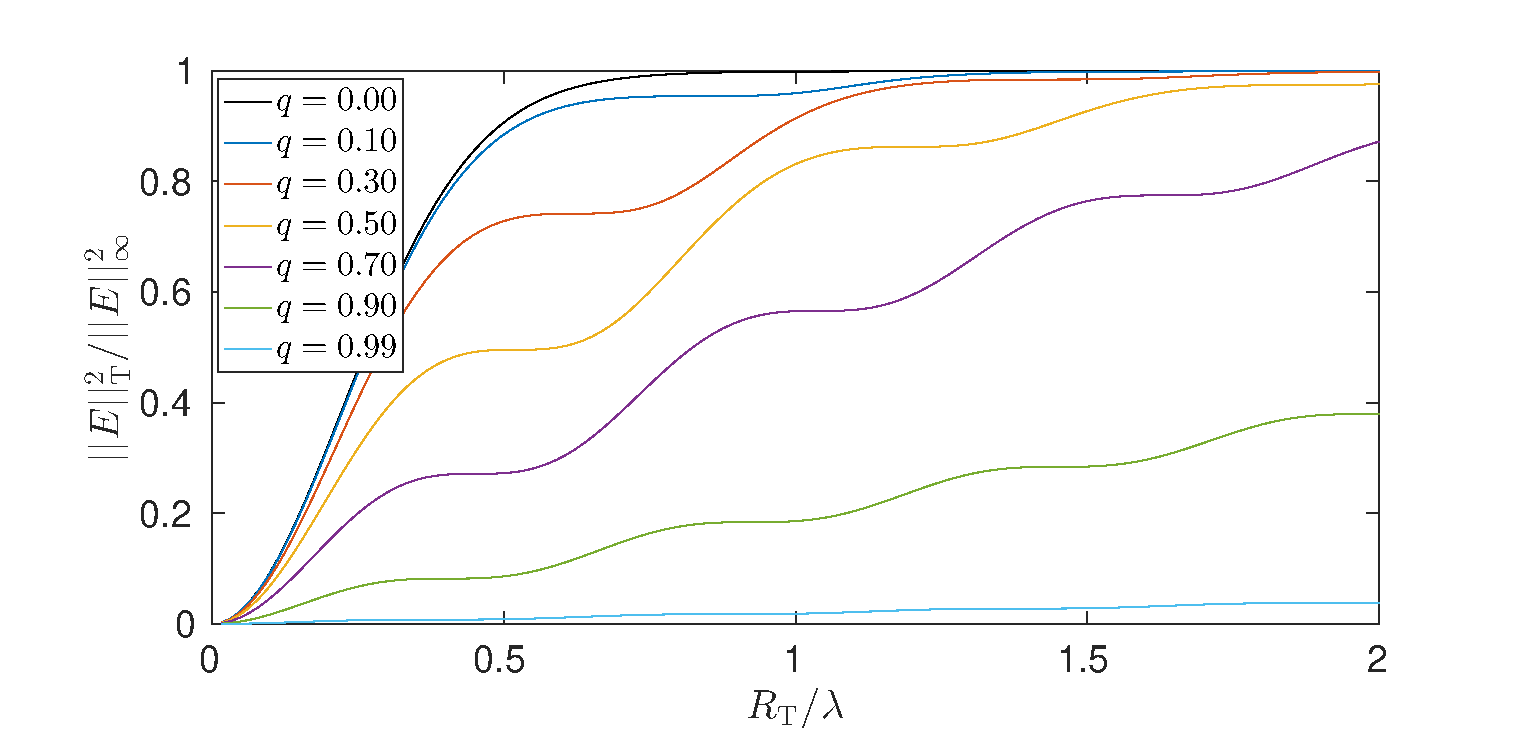
\includegraphics[width=18cm]{ring_T-infty_L1000.eps}
}
\caption{Theoretical maximum of energy-quotient inside the tumor
  to all of real space, as a function of tumor size, $\RT$, measures
  in sortest wavelengths, $\lambda$.}
\label{fig:T-infty}
\end{figure}

\begin{figure}\centering
\centerline{ % centers figures larges than 1\textwidth
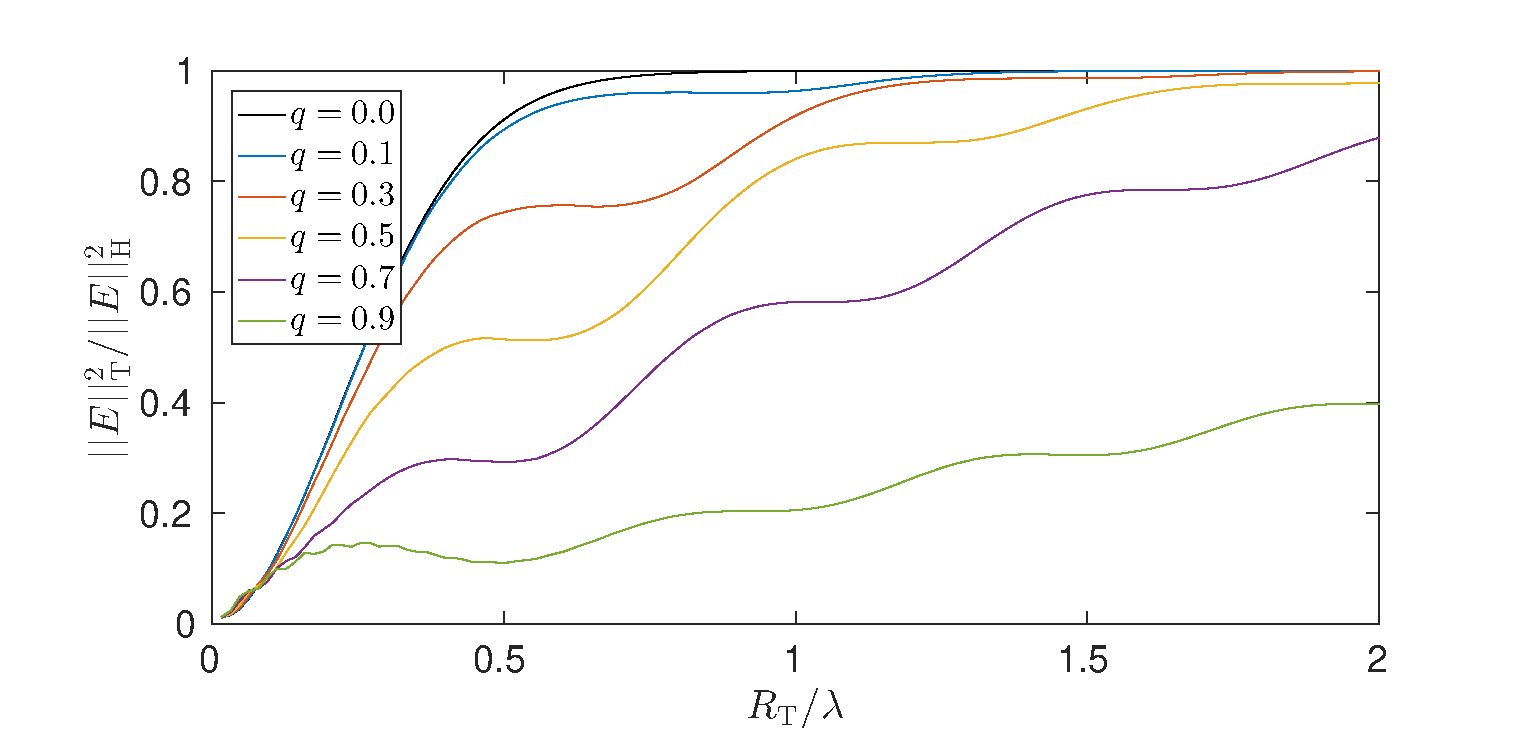
\includegraphics[width=18cm]{ring_T-H_L1000.eps}
}
\caption{Theoretical maximum of energy-quotient inside the tumor
  to a head around the tumor, as a function of tumor size, $\RT$,
  measures in sortest wavelengths, $\lambda$. Both the tumor and the
  head are circular discs of radius $\RT$ and $\RH$ respectively;
  $\RH=10RT$ was used for these graphs.}
\label{fig:T-infty}
\end{figure}

%%%%%%%%%%%%%%%%%%%%%%%%%%%%%%%%%%%%%%%%%%%%%%%%%%%%%%%%%%%%%%%%%%%%%%
\section{Discussion and further developments}
\label{ch:discussion}
\subsection{SAR}
\todo[inline]{May need some grooming to be presentable and shouldn't really be put here}
\newtheorem{theorem}{Theorem}
In hyperthermia treatment a good indicator for the temperature increase is the SAR-value (Specific Absorbation Rate), measured in [W/kg]:
\begin{equation*}
\text{SAR}(\vb*x)=\frac{\langle \vb*J(\vb*x,t)\cdot \vb*E(\vb*x,t) \rangle_t}{\rho(\vb*x)},
\end{equation*}
that is, a time average of the scalarproduct between the current density $\vb*J(\vb*x,t)$ and the electric field $\vb*E(\vb*x,t)$ divided by the density of the material $\rho(\vb*x)$. Due to Ohm's law this is simply a weighted version of the intensity $I=\abs{\vb*E}^2$. However, due to the time-averaging for multiple frequencies it can be shown that
\begin{equation}
\text{SAR}(\vb*x)=\sum_i\text{SAR}_i(\vb*x),         %\frac{1}{2}\sum_i\frac{\re[\sigma_i(\vb*x)\abs{\vb*E}^2]}{\rho(\vb*x)}
\end{equation}
that is a sum over the contribution from each frequency. In other words, when time-averaging there is no interference between different frequencies.
Since a finite energy will always be applied, all possible solutions will be a convex combination of the contribution for each frequency. And due to the linearity over frequencies, any convex goalfunction $G(\text{SAR})$ will be convex in the frequencies and a powerful theorem from convex optimization can be applied:
\begin{theorem}
 Let $f$ be a convex function defined on a convex set $X$. Then any local minima of $f$ is also a global minima on $X$.
\end{theorem}
This implies that the minimum of $G$ is obtained with only the frequency $\omega_j$ that gives the smallest contribution to $G$.

For a large family of goalfunctions the optimum is therefore obtained for a single frequency. In particular, any linear goalfunction is also convex and the main goalfunction used in this paper, \eqref{eq:energy_frac_final} would be optimized\footnote{the inverse of it would be minimized} by a single frequency if applied to SAR. 

%%%%%%%%%%%%%%%%%%%%%%%%%%%%%%%%%%%%%%%%%%%%%%%%%%%%%%%%%%%%%%%%%%%%%%
\section{Conclusions}





%%%%%%%%%%%%%%%%%%%%%%%%%% The bibliography %%%%%%%%%%%%%%%%%%%%%%%%%%
%\newpage
%% This bibliography ueses BibTeX
\bibliographystyle{ieeetr}
\bibliography{references}%requires a file named 'references.bib'
%% Citations are as usual: \cite{example_article}

%%%%%%%%%%%%%%%%%%%%%%%%%%%%% Appendices %%%%%%%%%%%%%%%%%%%%%%%%%%%%%
\clearpage %% on a new page 
\appendix  %% This will change the page numbering to A1, A2, A3, ...;
           %% and also change the sections to A, A.1, ...; B, B.1, ...


%%%%%%%%%%%%%%%%%%%%%%%%%%%%%%%%%%%%%%%%%%%%%%%%%%%%%%%%%%%%%%%%%%%%%%
\section{Numerical implementation of the 
Landau-Pollack-Slepian Theory}

In the previous section we have been occupied by integral eigenvalue
equations of the form
\begin{equation} %\label{eq:int-eig}
\lambda E(k) 
= \oldint_{\Omega} \rd^D{k}\, K(k, k') E(k')
\qcomma k, k'\in\Omega.
\end{equation}
We have also put down some work to reduce higher-dimensional
integrals to one-dimensional ones
\begin{equation} \label{eq:int-eig}
\lambda \psi(k) 
= \oldint_{I} \rd{k}\, K(k, k') \psi(k'),
\end{equation}
where the integration is now over an interval 
$I=[\alpha, \beta]$. This was done so that the numerical method
presented here could be applied. 


\subsection{Discretization of the integral equation}
The integral can be discretized according to
\begin{equation} \label{eq:inttosum}
\begin{aligned}
\oldint_I\rd{k} &\to \sum_{n=1}^N\Delta{k}
=\frac{\abs{I}}{N} \sum_{n=1}^N,\\
\psi(k) \to \psi_n = \psi(k_n) &\qcomma
K(k, k') \to K_{m, n} = K(k_m, k_n),
\end{aligned}
\end{equation}
where $\abs{I}=\beta-\alpha$ is the size of the interval $I$.
With these discretizations, \eqref{eq:int-eig} discretizes to
\begin{equation}
\lambda\Psi_m = \frac{\abs{I}}{N} \sum_{n=1}^N K_{m, n} \Psi_n
\end{equation}
which is just a matrix eigenvalue equation
\begin{equation} \label{eq:mtx-eig}
\Lambda \Psi = \mathsf{K}\Psi,
\end{equation}
where $\Lambda=N/\abs{I}\lambda$ and $\mathsf{K}$ is the $N\times N$ matrix
whose element $(m, n)$ is $K_{m, n}$. From here, there are many high
performance linear algebra libraries to find the eigenvalues and
eigenvector to \eqref{eq:mtx-eig} numerically. 

%\subsubsection{Symmetrization }
%We can also
Note that some effort was put into making the integral
kernel symmetric. This not only has the effect of guarateeing that the
eigenvectors of different eigenvalues will be orthogonal, but is also
beneficial to most numerical methods to find eigenvalues. 


% \subsubsection{Physical interpretation}
% An interesting physical interpretation of the discretization is that
% the operation \eqref{eq:inttosum} can be viewed as introducing
% \begin{equation}
% \Delta{k}\qty[\delta(k-k_0) + \delta(k-k_1) +\ldots+\delta(k-k_N)]
% \end{equation}
% into the integral, and effectively limiting the frequencydomain
% $\Omega$ to the dicrete frequencies $k_n$. 

% This idea could possibly be more cloesly related to reality, where the
% differnt antennas only transmitts in certain dicrete frequencies. And
% thus the discretized eigenvalue problem gives the theoretical maximum
% energy in a bounded region in space from a signal restriced to the
% chosen frequencies. 
% It is however worth pointing out that this result has only been proven
% for the 1D case\cite{PSWF-V_1978}, but there is no reason to believ
% that the discetized version cannot be extended to higher dimension
% like in the continuous case. 


\subsection{Justification of the numerical method}

\begin{table}

\centering
\caption{Table of eigevalues to the 2D disc of frequencies, as given
  by Slepian in \cite{PSWF-IV_1964}, $\lambda$, and numerically
  calculated using the method of this section, $\hat\lambda$; also the
  relative discrepancies between Slepian's method and this is given as
  $(\hat\lambda-\lambda)/\lambda$. The numerical values have been
  calculated using both the algorithem for only the full disc, and
  also using the algorithm for a circle ring with $q=1/L$.
}
\label{tab:just}
\begin{tabular}{|r|c|c|c|c|c|}\cline{2-6}
\multicolumn{1}{c|}{}
&Slepian\cite{PSWF-IV_1964}&
\multicolumn{2}{|c|}{Disc, numerical ($L=5000$)}&
\multicolumn{2}{|c|}{Ring, numerical ($L=1000$)}
\\ \hline
$c$\phantom{1.}&$\lambda$
&$\hat\lambda$&$(\hat\lambda-\lambda)/\lambda$
&$\hat\lambda$&$(\hat\lambda-\lambda)/\lambda$
\\ \hline
  0.1 & 2.4968775e-3 & 
2.49787510e-03 &\bf\phantom{-}4.0e-4&  
2.49687188e-03 &\bf-2.3e-6
\\ \hline
  0.5 & 6.0585348e-2 & 
6.06088302e-02 &\bf\phantom{-}3.9e-4&  
6.05834074e-02 &\bf-3.2e-5
\\ \hline
  1.0 & 2.2111478e-1 & 
2.21192655e-01 &\bf\phantom{-}3.5e-4&  
2.21087997e-01 &\bf-1.2e-4
\\ \hline
  1.5 & 4.2951906e-1 & 
4.29646579e-01 &\bf\phantom{-}3.0e-4&  
4.29407932e-01 &\bf-2.5e-4
\\ \hline
  2.0 & 6.2963045e-1 & 
6.29775619e-01 &\bf\phantom{-}2.3e-4&  
6.29363231e-01 &\bf-4.2e-4
\\ \hline
  3.0 & 8.8705036e-1 & 
8.87143325e-01 &\bf\phantom{-}1.0e-4&  
8.86395173e-01 &\bf-7.3e-4
\\ \hline
  5.0 & 9.9534230e-1 & 
9.95350350e-01 &\bf\phantom{-}8.1e-6&  
9.94366440e-01 &\bf-9.8e-4
\\ \hline
 10.0 & 9.9999957e-1 & 
9.99999399e-01 &\bf\phantom{}-1.7e-7&  
9.98997959e-01 &\bf-1.0e-3
\\ \hline
\end{tabular}
\end{table}


%%%%%%%%%%%%%%%%%%%%%%%%%%%%%%%%%%%%%%%%%%%%%%%%%%%%%%%%%%%%%%%%%%%%%%
\end{document}%% ^ ^ ^ ^ ^ ^ ^ ^ ^ ^ ^ ^ ^ ^ ^ ^ ^ ^ ^ ^ ^ ^ ^ ^ ^ ^ ^
%%%%%%%%%%%%%%%%%%%%%%%%%%%%%%%%%%%%%%%%%%%%%%%%%%%%%%%%%%%%%%%%%%%%%%




%%%%  Some (useful) templates


%% På svenska ska citattecknet vara samma i både början och slut.
%% Använd två apostrofer: ''.


%% Including PDF-documents
\includepdf[pages={1-}]{filnamn.pdf} % NO blank spaces in the file name

%% Figures (pdf, png, jpg, ...)
\begin{figure}\centering
\centerline{ % centers figures larges than 1\textwidth
\includegraphics[width=.8\textwidth]{file_name.pdf}
}
\caption{}
\label{fig:}
\end{figure}

%% Figures from xfig's "Combined PDF/LaTeX"
\begin{figure}\centering
\resizebox{.8\textwidth}{!}{\input{file_name.pdf_t}}
\caption{}
\label{fig:}
\end{figure}


%% If you want to add something to the ToC
%% (Without having an actual header in the text.)
\stepcounter{section} %For example a 'section'
\addcontentsline{toc}{section}{\Alph{section}\hspace{8 pt}Labblogg} 

